\setAuthor{Valter Kiisk}
\setRound{lahtine}
\setYear{2019}
\setNumber{G 2}
\setDifficulty{2}
\setTopic{TODO}

\prob{Pumpjaam}
\begin{wrapfigure}[7]{r}{0.45\textwidth}
    \vspace{-23pt}
	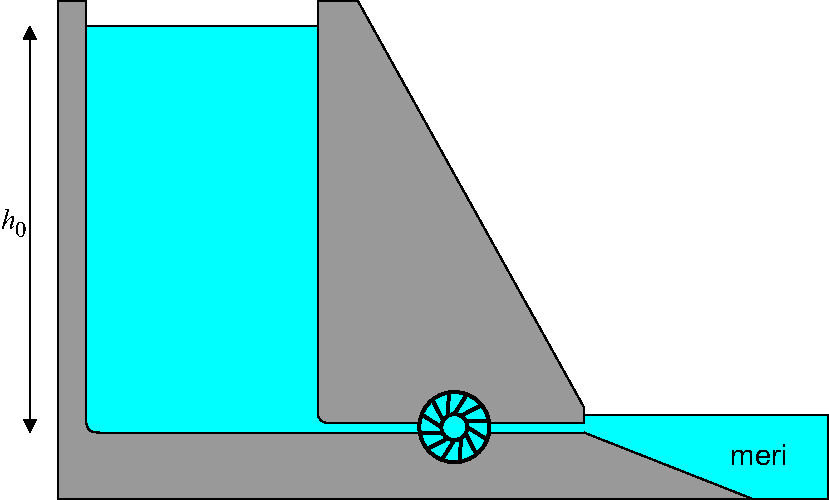
\includegraphics[width=0.45\textwidth]{2019-lahg-02-yl.pdf}
\end{wrapfigure}

Arenenud riikides on elektrienergia tarbimine, võrrelduna riigi pindalaga, suurusjärgus \SI{100}{\kilo\watt\per\kilo\meter\squared}. Joonisel on kujutatud teatava pump-hüdroakumulatsiooni elektrijaama skeem. Eeldame, et alumiseks reservuaariks on meri (mille tase püsib praktiliselt muutumatu) ja ülemise reservuaari põhi ulatub praktiliselt merepinna tasemeni. Elektrienergia ületootmise ajal pumbatakse merevett ülemisse reservuaari kuni kõrguseni $h_0=\SI{100}{m}$. Energiadefitsiidi ajal toimib sama süsteem hüdroelektrijaamana. Ignoreerides energia konverteerimis- ja ülekandekadusid, kui suure osa riigi pindalast peaks sellised pumpjaamad (st ülemise reservuaari pindala) moodustama, et muude elektritootjate äralangemisel kindlustada elektrienergia varu 24 tunniks?


\hint

\solu
Olgu reservuaari pindala $S$. Vee mass on $m=\rho V=\rho h_0S$. Selle masskese on tõstetud kõrgusele $h=h_0/2$, seega potentsiaalne energia on $mgh=\frac{1}{2}\rho gh_0^2S$ ja energia pinnaühiku kohta
\[
w_s=\frac{1}{2}\rho gh_0^2\approx \SI{49}{\mega\joule\per\meter\squared}\approx\SI{13.6}{kWh\per\meter\squared}.
\]

Energiavajaduse rahuldamiseks on vaja keskmist energiatihedust
\[
w_t=\SI{100}{\kilo\watt\per\kilo\meter\squared}\cdot \SI{24}{\hour}=\SI{2400}{kWh\per\kilo\meter\squared}=\SI{0.0024}{kWh\per\meter\squared}.
\]
Otsitav suurus on ilmselt $w_t/w_s\approx \num{1.8e-4}$.
\probend